\chapter{Simulations}
\label{sec:simulations}

We evaluate the \texttt{LASER} %and $H_\infty$
 algorithm on four synthetic datasets.
We set $T=2000$ and $d=20$. For all datasets, the
inputs $\mathbf{x}_t\in\reals^{20}$ were generated such that
the first ten coordinates were grouped into five groups of size
two. Each such pair was drawn from a $45^\circ$ rotated Gaussian
distribution with standard deviations $10$ and $1$. The remaining $10$
coordinates were drawn from independent Gaussian distributions
$\norm\paren{0,2}$. The first synthetic dataset was
generated using a sequence of vectors $\vui{t}\in\reals^{20}$ for
which the only non-zero coordinates are the first two, where their
values are the coordinates of a unit vector that is rotating with a
constant rate (linear drift). Specifically, we have $\Vert\vui{t}\Vert=1$ and the
instantaneous drift $\Vert\vui{t}-\vui{t-1}\Vert$ is constant.  The
second synthetic dataset was generated using a sequence
of vectors $\vui{t}\in\reals^{20}$ for which the only non-zero
coordinates are the first two. This vector in $\reals^2$ is of unit
norm $\Vert\vui{t}\Vert=1$ and rotating in a rate of $t^{-1}$ (sublinear drift). In
addition every $50$ time-steps the two-dimensional vector defined
above was ``embedded'' in different pair of coordinates of the
reference vector $\vui{t}$, for the first $50$ steps it were
coordinates $1,2$, in the next $50$ examples, coordinates $3,4$, and
so on. This change causes a switch in the reference vector $\vui{t}$.
For the first two datasets we set $\yi{t}=\vxti{t}\vui{t}$ (linear data).
The third and fourth datasets are the same as first and second except we set $\yi{t}=\vxti{t}\vui{t}+n_t$ where
$n_t\sim\norm\paren{0,0.05}$ (noisy data).

We compared five algorithms: NLMS (normalized least mean
square)~\citep{Bershad,Bitmead} which is a state-of-the-art first-order
algorithm, AROWR (AROW for Regression)~\citep{CrammerKuDr09},
ARCOR~\citep{VaitsCr11}, CR-RLS~\citep{Salgado,Goodwin,Chen} and our \texttt{LASER} % and $H_\infty$
algorithm. The
algorithms' parameters were tuned using a single random sequence. We
repeat each experiment $100$ times reporting the mean cumulative
square-loss.

%
\begin{center}
\begin{figure}[t!]
\subfigure{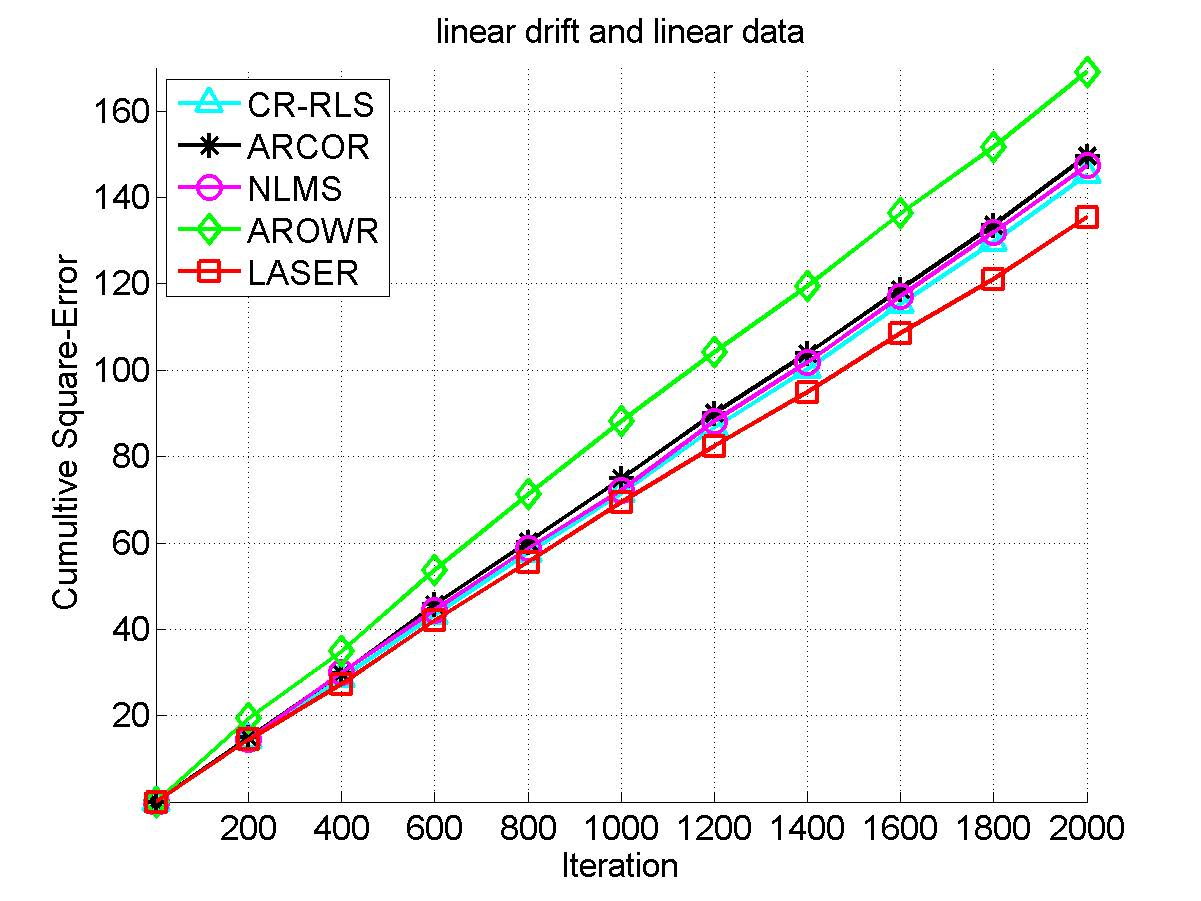
\includegraphics[width=0.50\textwidth]{figs/linear_drift_linear_data.pdf}}
\subfigure{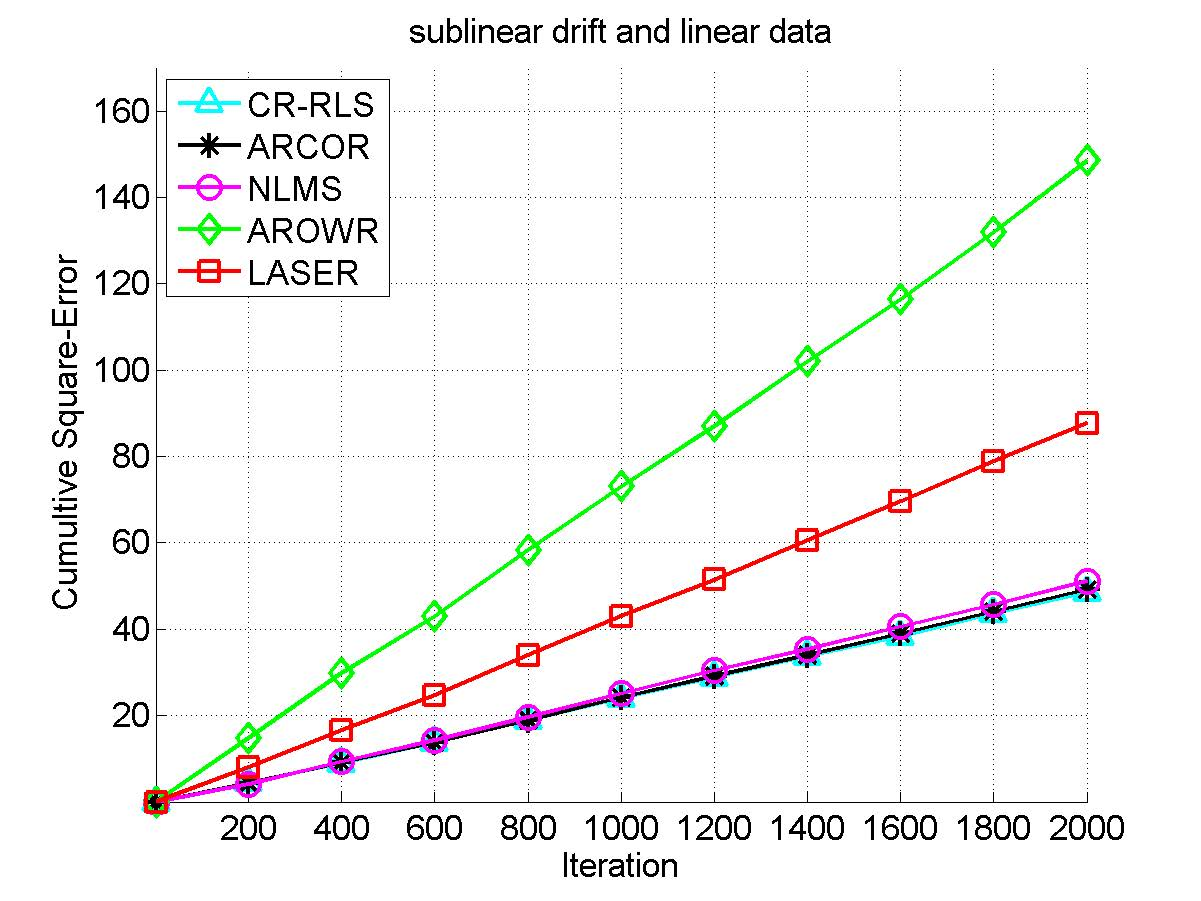
\includegraphics[width=0.50\textwidth]{figs/sublinear_drift_linear_data.pdf}}
\subfigure{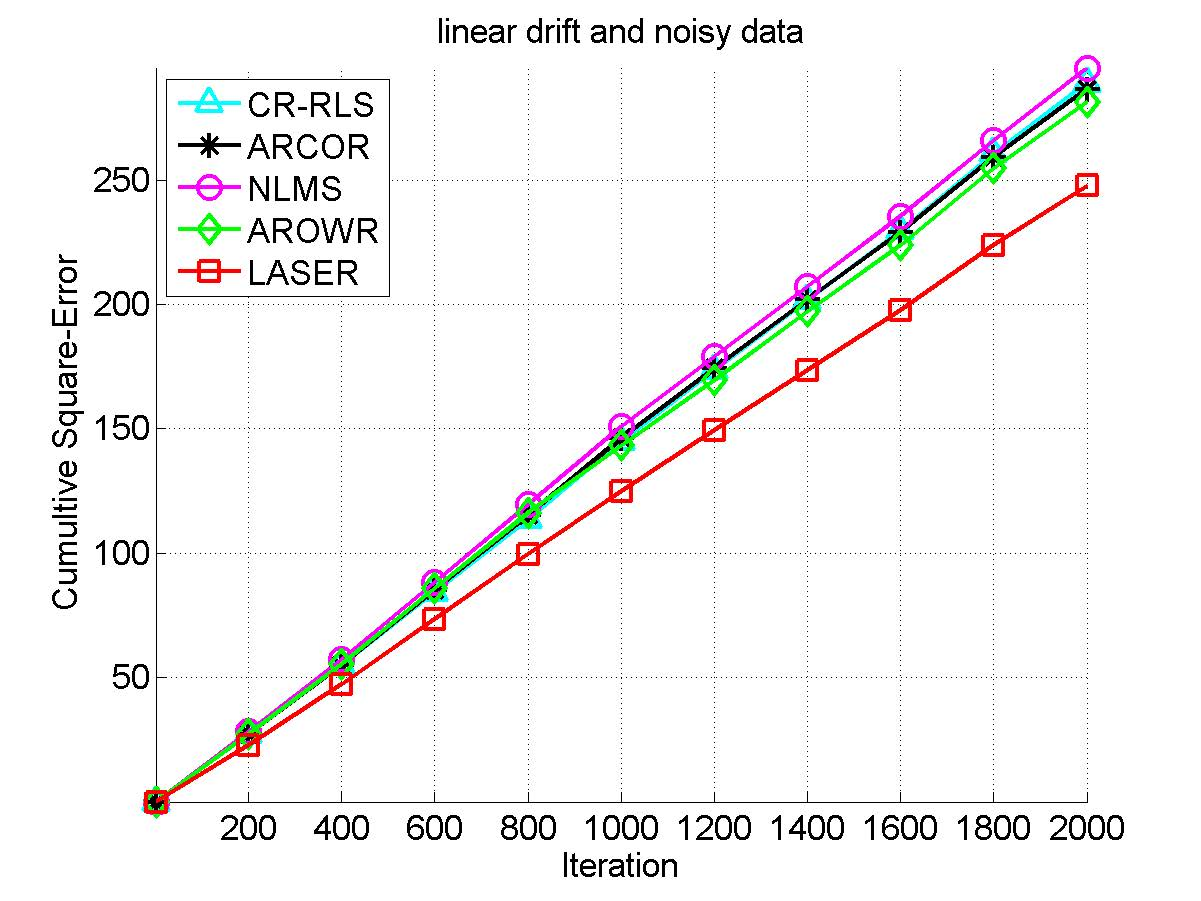
\includegraphics[width=0.50\textwidth]{figs/linear_drift_noisy_data.pdf}}
\subfigure{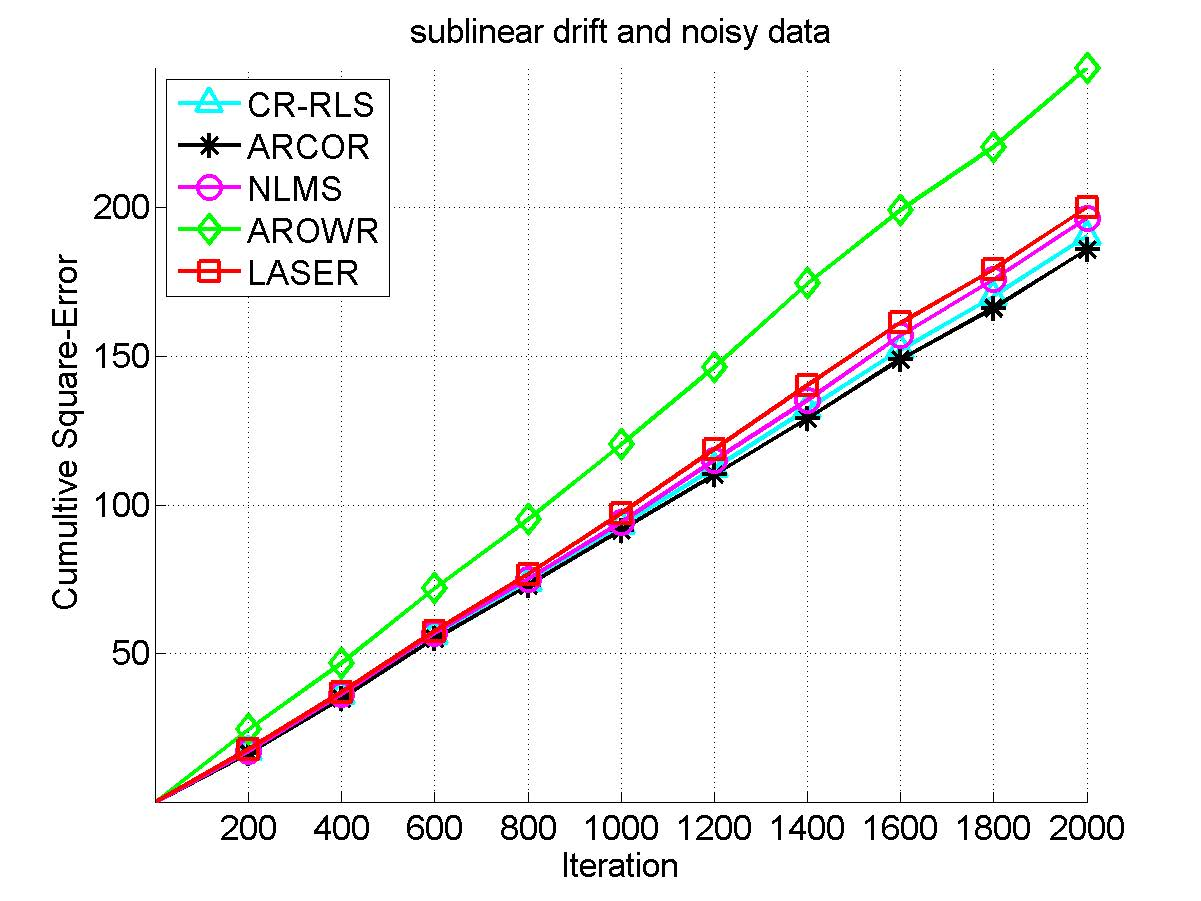
\includegraphics[width=0.50\textwidth]{figs/sublinear_drift_noisy_data.pdf}}
\caption{Cumulative squared loss for NLMS, AROWR, ARCOR,
  CR-RLS and LASER vs iteration. % Top left - linear drift and linear data, top right - sublinear drift and linear data,
  %bottom left - linear drift and noisy data, bottom right - sublinear drift and noisy data.
  }
\label{fig:sims}
\end{figure}
\end{center}
%

The results for the first dataset are summarized in the top-left plot of
\figref{fig:sims}.
For this dataset
AROWR performs the worst, since it converges very fast and does not
allow the ability of tracking changes in data. The ARCOR algorithm for
this dataset performs relatively bad, this is due to the fact that it
is designed for sublinear amount of data drift, while this dataset has
linear drift level, which is the worst case assumed by \texttt{LASER}. CR-RLS
and NLMS show better results, since they both don't make assumptions
on the drift level. CR-RLS performs a little bit better than NLMS
since it has faster learning rate due to the use of second order
information. Finally, LASER %and $H_\infty$
performs the best as expected. It has a good tracking ability, fast learning rate and it is designed to perform well in severe conditions like linear non-stationarity of the data. %, while $H_\infty$ outperforms LASER as expected when the data is close to be linear ($\yi{t}=\vxti{t}\vui{t}$).
Similar results we get for the third dataset (bottom-left plot of \figref{fig:sims}).

For the second and fourth datasets (right plots of
\figref{fig:sims}), where we have sublinear drift level, we get that ARCOR
outperforms \texttt{LASER} since it is especially designed for sublinear amount
of data drift.%, yet, $H_\infty$ outperforms ARCOR.

%For the third and fourth datasets (bottom plots of \figref{fig:sims}), where we added noise to labels, the performance of $H_\infty$ degrades, as expected from our discussion in \chapref{H8_sec}.




